One area identified for potential reinforcement learning application is in the design of a fault tolerant controller.  Fault tolerant controllers activate when a process fault occurs, rendering normal controllers useless [citation required]. The objective of fault tolerant controllers are to guide the process out of the fault situation safely.  Subsequently, process engineers can diagnose the problem and re-activate the normal process controllers.  

Farivar and Ahmadabadi (2015) has designed fault tolerant controllers using reinforcement learning for a class of unknown linear systems \cite{ahmad}.  Zhang and Gao (2018) applied reinforcement learning fault tolerant controllers to flux cored wired systems \cite{zhang_gao}.  In this project, a reinforcement learning fault tolerant controller will be built for the mitigation of flooding in an industrial distillation tower. 

Flooding is one of the most common problems in industrial distillation towers.  Flooding causes XXX damage and XXX. Reinforcement learning can be used to create an experience driven, online learning fault tolerant controller to mitigate damage caused by flooding in distillation towers.  In this chapter, the process will first be introduced. Then, common faults will be introduced into the system.  Following that, PID, MPC and RL will all be used to try to guide the system out of the fault situation.  Finally, the performance of each controller will be compared.

\section{Process Introduction}
The Wood-Berry distillation tower, located in the Unversity of Alberta, will be used to compare the performance between PID, MPC, and RL controllers in a fault positive scenario.  

\subsection{Process Description}
Distillation is the process of separating a liquid or vapour mixture of two or more components into desirable purities through the addition or removal of heat. The fundamental theory of distillation is that low boiling point components are richer in the vapour of a boiling mixture, while the liquids would contain more of the less volatile components \cite{distillation_intro}.  Liquids exit the bottom of the distillation tower and is sent to a reboiler, where heat is added to vaporize any straggling high volatility product to ensure maximum separation. Similarly, vapour from the top of the tower is sent to a condenser, where heat is removed and additional low volatility components may be recovered. The condensed vapour is collected in the reflux drum, and will be recycled back into the distillation tower. Typically, distillation columns are large vertical drums with evenly spaced trays to enhance separation of the vapour and liquid components \cite{mpc_for_distillation_tower}.  The tower is separated into two sections.  The rectifying section is located between the feed tray and the top of the column and aims to concentrate light components in the vapour phase.  Moreover, the stripping section is located between the feed tray and the column bottom and is used to concentrate the heavier components in the liquid phase \cite{henry_distillation}.

A process flow diagram of the Wood-Berry tower is shown in Figure \ref{fig: woodberry}.  It contains one feed stream and two outlet streams.  Commonly, the feed stream is characterized by the inlet mol composition, $Z_f$.  The top product, also called distillate, is characterized by mass fraction, $X_D$.  The bottom product is characterized by mass fraction, $X_B$.  The process has two control inputs and two outputs. The control inputs of the system are the reflux and steam flow rates, $R$ and $S$.  The outputs are the distillate and bottoms product mass compositions, $X_D$ and $X_B$.

\begin{figure}[h]
    \centering
    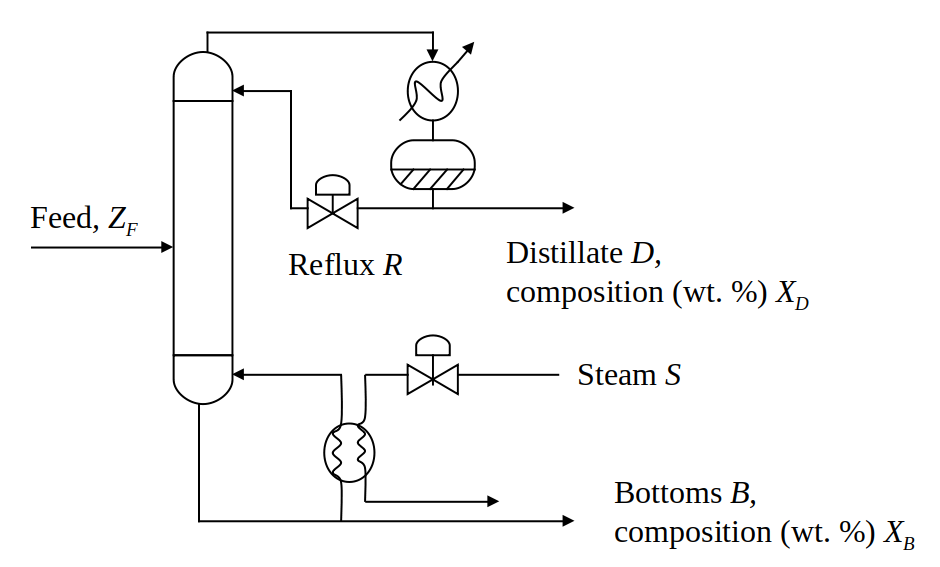
\includegraphics[scale=0.45]{images/woodberry.png}
    \caption{A schematic diagram of a binary distillation tower.  Original figure from Dr. Seborg from UC Santa Barbara.}
    \label{fig: woodberry}
\end{figure}

In the Wood-Berry distillation tower, the goal is to completely separate methanol and water.  Methanol has a boiling point of 64.7 \textdegree C whereas pure liquid water has a boiling point of 100 \textdegree C \cite{sonntag_thermo}. Thus, making methanol the distillate and water is the bottoms product. Additional detailed information about the operation and inner workings of distillation towers can be found in \cite{henry_distillation}.  

\subsection{Wood-Berry Models}
The transfer functions that realize  the Wood-Berry distillation tower is given in Equation \ref{eq: woodberry_tf} \cite{mpc_for_distillation_tower}.

\begin{equation}
    \centering
    \begin{bmatrix}
        Y_1(s) \\
        Y_2(s) 
    \end{bmatrix}
    =
    \begin{bmatrix}
        G_{11}  & G_{12} \\
        G_{21}  & G_{22}
    \end{bmatrix}
    \begin{bmatrix}
        u_1(s) \\
        u_2(s)
    \end{bmatrix}
    \label{eq: woodberry_tf}
\end{equation}

where: \\
\begin{center}
    $
    \large
    \begin{matrix}
        G_{11} = \frac{12.8e^{-s}}{16.7s + 1}     &     G_{12} = \frac{-18.9e^{-3s}}{21s + 1} \\
        G_{21} = \frac{6.6e^{-7s}}{10.9s + 1}     &     G_{22} = \frac{-19.4e^{-3s}}{14.4s + 1}
    \end{matrix}
    $
\end{center}

Due to the difficulty of transfer function simulations in Python, the model was converted into state space form.  After conversion, two control loops had to be developed to realize the system because of inconsistencies in the process time delay for $u_1$.  Equations \ref{eq: x_ss_eq1} and \ref{eq: x_ss_eq2} are the state space models for the distillate and bottoms compositions, respectively.

\begin{equation}
    \centering
    \begin{bmatrix}
        \dot{x_1} \\
        \dot{x_2} \\
        \dot{x_3} \\
        \dot{x_4} 
    \end{bmatrix}
    =
    \begin{bmatrix}
        -0.0599     &     0     &     0     &     0 \\
        0           &  -0.0917  &     0     &     0 \\
        0           &     0     &   -0.0476 &     0 \\
        0           &     0     &     0     &  -0.0694
    \end{bmatrix}
    \begin{bmatrix}
        x_1 \\
        x_2 \\
        x_3 \\
        x_4 
    \end{bmatrix}
    +
    \begin{bmatrix}
        1     &     0  \\
        1     &     0  \\
        0     &     1  \\
        0     &     1
    \end{bmatrix}
    \begin{bmatrix}
        u_1(t - 1) \\
        u_2(t - 3)
    \end{bmatrix}
    \label{eq: x_ss_eq1}
\end{equation}

\begin{equation}
    \centering
    Y_1(t) =  
    \begin{matrix}
        [0.7665 & 0 & -0.9 & 0]
    \end{matrix}
    \begin{matrix}
        [x_1 & x_2 & x_3 & x_4]^T
    \end{matrix}
\end{equation}

\begin{equation}
    \centering
    \begin{bmatrix}
        \dot{x_1} \\
        \dot{x_2} \\
        \dot{x_3} \\
        \dot{x_4} 
    \end{bmatrix}
    =
    \begin{bmatrix}
        -0.0599     &     0     &     0     &     0 \\
        0           &  -0.0917  &     0     &     0 \\
        0           &     0     &   -0.0476 &     0 \\
        0           &     0     &     0     &  -0.0694
    \end{bmatrix}
    \begin{bmatrix}
        x_1 \\
        x_2 \\
        x_3 \\
        x_4 
    \end{bmatrix}
    +
    \begin{bmatrix}
        1     &     0  \\
        1     &     0  \\
        0     &     1  \\
        0     &     1
    \end{bmatrix}
    \begin{bmatrix}
        u_1(t - 7) \\
        u_2(t - 3)
    \end{bmatrix}
    \label{eq: x_ss_eq2}
\end{equation}

\begin{equation}
    \centering
    Y_2(t) =  
    \begin{matrix}
        [0 & 0.6055 & 0 & -1.3472]
    \end{matrix}
    \begin{matrix}
        [x_1 & x_2 & x_3 & x_4]^T
    \end{matrix}
\end{equation}

\subsection{Model Validation}

To ensure the state space model is equivalent to the original transfer function model, step tests were conducted on both systems.  Explain step test and inputs...

The steady state problem was also calculated to ensure simulations were giving correct results...

\section{Fault in the System}

\section{Controlling using PID}
A PI controller was selected instead of a P or PID controller, because PI controllers are shown to achieve superior control performances compared to their counterparts \cite{PI_controller}.

\section{Controlling using MPC}
\section{Controlling using Reinforcement Learning}
\section{Comparison of Performance}